\chapter{Augmenting Data Structures}

Over the last few chapters you have built a fast, dependable machine. A red-black
tree gives you \texttt{INSERT}, \texttt{DELETE}, \texttt{SEARCH},
\texttt{MINIMUM}, \texttt{MAXIMUM}, \texttt{SUCCESSOR}, and
\texttt{PREDECESSOR}, every one of them in $O(\lg n)$ time, even in the worst
case, because the tree stays balanced. That is a versatile set of operations
at $O(\lg n)$ cost per query.

Real applications, however, rarely ask the exact question a standard
textbook data structure answers out of the box. A bank wants to know, ``how many of my
customers have a balance below this one?'' A scheduler wants to know, ``does any
meeting on the calendar overlap the slot 2:00--3:00?'' A median-tracking
dashboard wants to know, ``what is the 90th-percentile latency \emph{right now},
as requests stream in?'' None of these is plain \texttt{SEARCH}.

You have two options. You could invent a brand-new data structure from the
ground up for each new question --- exhausting, error-prone, and wasteful. Or you
could take a structure you already trust and \emph{teach it a new trick} by
storing a little extra information at each node. That second path is what this
chapter is about. It is called \emph{augmenting} a data structure, and once you
see how it works, you will start to spot opportunities for it everywhere.

\begin{intuitionbox}
Augmenting a data structure is like adding a mileage counter to a car you
already own. You do not rebuild the engine. You bolt on one small gauge, wire it
to something the car already does (turning the wheels), and make sure it stays
accurate as you drive. The hard part is never the gauge itself --- it is keeping
it correct every time the car moves.
\end{intuitionbox}

We will work through two flagship examples --- \emph{order-statistic trees}, which
answer ranking and percentile questions, and \emph{interval trees}, which answer
overlap questions --- and between them we extract the general recipe: a
short theorem that tells you exactly when augmentation is cheap and how to do it
without breaking what you already had.

\chapterline

\section{Warming Up: What Question Are We Even Asking?}

Suppose you have $n$ distinct numbers and you store them in a balanced binary
search tree. The tree already answers ``is $x$ present?'' and ``what is the
smallest element?'' Now imagine someone hands you these two new requests:

\begin{itemize}
  \item \textbf{\texttt{SELECT}$(i)$:} return the element with the $i$th smallest
    key. If $i = 1$ you want the minimum; if $i = n$ you want the maximum; if
    $i = \lceil n/2 \rceil$ you want the median.
  \item \textbf{\texttt{RANK}$(x)$:} given a node $x$ in the tree, return its
    position in sorted order. If $x$ holds the smallest key, its rank is $1$.
\end{itemize}

These two are inverses of each other. \texttt{SELECT} goes from a \emph{position}
to an \emph{element}; \texttt{RANK} goes from an \emph{element} to its
\emph{position}. Together they are called \emph{order-statistic} queries, because
the $i$th smallest element is also called the $i$th \emph{order statistic} of the
set. (You met order statistics back in Chapter~9; there we found a
single one in linear time on a static array. Here we want a \emph{dynamic} set
that supports insert and delete \emph{and} answers order-statistic queries fast.)

\begin{focusbox}
Hold onto this distinction:
\texttt{SELECT}$(i)$ = ``give me the $i$th smallest'' (position $\to$ element),
\texttt{RANK}$(x)$ = ``where does $x$ sit in sorted order?'' (element $\to$
position). Everything in the first half of this chapter is about answering both
in $O(\lg n)$ time on a set that keeps changing.
\end{focusbox}

The crude attempt: walk the tree in sorted order (an in-order traversal),
counting as you go, and stop at the $i$th node. That works, but it costs
$\Theta(n)$ in the worst case --- you might walk the whole tree. We did all that
work to get $O(\lg n)$ operations, and now a single query throws it away. We can
do far better, and the trick is to store one extra number per node.

\section{Order-Statistic Trees: The Idea}
\label{ch14:sec-ostree}

Take an ordinary red-black tree. At every node $x$, add one new field,
\texttt{$x$.size}, defined as the number of nodes in the subtree rooted at $x$,
\emph{including $x$ itself}. To make the bookkeeping uniform, we let the sentinel
\texttt{NIL} (the stand-in leaf at the bottom) have size $0$. Then for every real
node the field obeys a clean local rule:
\[
  x.\mathit{size} \;=\; x.\mathit{left}.\mathit{size} \;+\; x.\mathit{right}.\mathit{size} \;+\; 1.
\]
In words: the size of your subtree is the size of your left subtree, plus the
size of your right subtree, plus one for yourself. That ``$+1$'' is you.

\begin{intuitionbox}
Think of \texttt{size} as each node knowing the headcount of the family living
beneath it (itself included). The root knows the whole population, $n$. A leaf
knows just itself, $1$. Importantly, a node can compute its own headcount knowing
\emph{only} the headcounts of its two children --- it never has to look further
down. That ``I only need my kids'' property is what will make updates cheap.
\end{intuitionbox}

Here is a small tree of seven keys, with each node labelled \emph{key /
size}. Spend a moment checking the rule at every node.

\begin{center}
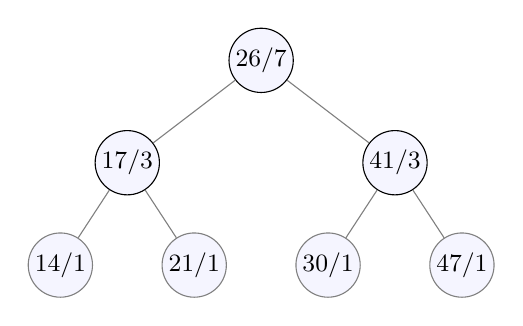
\begin{tikzpicture}[
  every node/.style={draw, circle, minimum size=8mm, inner sep=1pt,
    font=\small, fill=blue!4},
  level distance=13mm,
  level 1/.style={sibling distance=34mm},
  level 2/.style={sibling distance=17mm},
  edge from parent/.style={draw, gray}]
  \node {$26/7$}
    child {node {$17/3$}
      child {node {$14/1$}}
      child {node {$21/1$}}
    }
    child {node {$41/3$}
      child {node {$30/1$}}
      child {node {$47/1$}}
    };
\end{tikzpicture}
\end{center}

Check the root: its left subtree (rooted at $17$) has size $3$, its right subtree
(rooted at $41$) has size $3$, plus itself makes $3+3+1 = 7$. Good. Check node
$17$: $1 + 1 + 1 = 3$. Good. Every leaf has two \texttt{NIL} children of size $0$,
so $0 + 0 + 1 = 1$. The rule holds everywhere.

\subsection{\texttt{SELECT}: finding the $i$th smallest}

Now watch how that one number lets you home in on the $i$th smallest element
without ever scanning. Stand at a node $x$. Let
\[
  r \;=\; x.\mathit{left}.\mathit{size} + 1.
\]
This $r$ is the rank of $x$ \emph{within the subtree rooted at $x$}: everything in
$x$'s left subtree is smaller than $x$, and there are
$x.\mathit{left}.\mathit{size}$ of them, so $x$ itself is the
$r$th smallest in its own subtree. Three cases:

\begin{itemize}
  \item If $i = r$, then $x$ \emph{is} the element you want. Done.
  \item If $i < r$, the element you want is smaller than $x$, so it lives in the
    left subtree. Recurse left, still looking for the $i$th smallest (the count
    is unchanged --- everything to the left is still to the left).
  \item If $i > r$, the element is bigger than $x$. Recurse right. But now you
    must \emph{subtract} the $r$ elements you have skipped over (everything in
    the left subtree, plus $x$ itself): in the right subtree you are now hunting
    for the $(i - r)$th smallest.
\end{itemize}

\begin{algorithm}[H]
\caption{\textsc{OS-Select}$(x, i)$ --- the $i$th smallest in the subtree at $x$}
\KwIn{a subtree root $x$, and an index $i$ with $1 \le i \le x.\mathit{size}$}
\KwOut{the node holding the $i$th smallest key in $x$'s subtree}
$r \gets x.\mathit{left}.\mathit{size} + 1$\;
\If{$i = r$}{\Return $x$\;}
\eIf{$i < r$}{
  \Return \textsc{OS-Select}$(x.\mathit{left},\, i)$\;
}{
  \Return \textsc{OS-Select}$(x.\mathit{right},\, i - r)$\;
}
\end{algorithm}

To answer a query on the whole tree, you call
\textsc{OS-Select}$(\mathit{root}, i)$.

\begin{labbox}
Let us find the \textbf{3rd smallest} in the seven-node tree above, by hand.
Call \textsc{OS-Select}$(\mathit{root}=26,\ i=3)$.

\textbf{Step 1.} At node $26$: left subtree (rooted at $17$) has size $3$, so
$r = 3 + 1 = 4$. We want $i = 3$. Since $3 < 4$, the answer is to the left.
Recurse into node $17$ with $i = 3$.

\textbf{Step 2.} At node $17$: left subtree (node $14$) has size $1$, so
$r = 1 + 1 = 2$. We want $i = 3$. Since $3 > 2$, go right and subtract:
recurse into node $21$ with $i = 3 - 2 = 1$.

\textbf{Step 3.} At node $21$: left subtree is \texttt{NIL}, size $0$, so
$r = 0 + 1 = 1$. We want $i = 1$. Since $1 = 1$, \textbf{return node $21$}.

Sanity check: the sorted keys are $14, 17, 21, 26, 30, 41, 47$. The 3rd smallest
is indeed $21$. We touched exactly $3$ nodes --- the height of the tree --- not all
seven.

\begin{center}
\begin{tikzpicture}[
  every node/.style={draw, circle, minimum size=8mm, inner sep=1pt,
    font=\small, fill=blue!4},
  visited/.style={fill=quotientorange!25, draw=quotientorange, line width=1pt},
  found/.style={fill=targetgreen!25, draw=targetgreen, line width=1.2pt},
  level distance=13mm,
  level 1/.style={sibling distance=34mm},
  level 2/.style={sibling distance=17mm},
  edge from parent/.style={draw, gray}]
  \node[visited] {$26/7$}
    child {node[visited] {$17/3$}
      child {node {$14/1$}}
      child {node[found] {$21/1$}}
    }
    child {node {$41/3$}
      child {node {$30/1$}}
      child {node {$47/1$}}
    };
\end{tikzpicture}
\end{center}

The shaded path is the only part of the tree \textsc{OS-Select} ever looks at:
$26$ (steer left), then $17$ (steer right), then $21$ (the green answer). The
four unshaded nodes are never visited.
\end{labbox}

\begin{trapbox}
The single most common bug is forgetting to subtract when you go right. If you
recurse right still asking for the $i$th smallest, you are now asking for the
$i$th smallest \emph{of the right subtree}, which is a completely different
element. You must shrink the target to $i - r$, because by stepping right you
have left $r$ smaller elements (the whole left subtree, plus $x$) behind you.
Trace the example again and watch where the $3 \to 1$ happens.
\end{trapbox}

Because the tree is balanced, its height is $O(\lg n)$, and
\textsc{OS-Select} descends one level per call, so a query costs $O(\lg n)$.

\subsection{\texttt{RANK}: where does this node sit?}

Now the inverse. Given a pointer to a node $x$, what is its position in the
sorted order of the \emph{whole} tree? Start with the rank of $x$ inside its own
subtree, namely $x.\mathit{left}.\mathit{size} + 1$, and then climb toward the
root. Each time you step up, ask: did I just come up from a right child? If so,
everything in that sibling-and-parent's left side, plus the parent itself, is
smaller than $x$ and has not yet been counted --- so add it in. If you came up from
a left child, you are still on the small side of that parent, so add nothing.

\begin{algorithm}[H]
\caption{\textsc{OS-Rank}$(T, x)$ --- the position of node $x$ in sorted order}
\KwIn{an order-statistic tree $T$ and a node $x$ in it}
\KwOut{the rank of $x$ among all keys of $T$ (so $1$ means smallest)}
$r \gets x.\mathit{left}.\mathit{size} + 1$\;
$y \gets x$\;
\While{$y \ne T.\mathit{root}$}{
  \If{$y = y.\mathit{parent}.\mathit{right}$}{
    $r \gets r + y.\mathit{parent}.\mathit{left}.\mathit{size} + 1$\;
  }
  $y \gets y.\mathit{parent}$\;
}
\Return $r$\;
\end{algorithm}

\begin{labbox}
Let us compute \textsc{OS-Rank} of node $21$ in the same tree, and confirm we get
$3$ back (the inverse of the previous lab).

\textbf{Start.} $x = 21$. Its left child is \texttt{NIL} (size $0$), so
$r = 0 + 1 = 1$. Set $y = 21$.

\textbf{Climb 1.} $y = 21$ is the \emph{right} child of its parent $17$. So add
the parent's left subtree (node $14$, size $1$) plus $1$ for the parent:
$r \gets 1 + 1 + 1 = 3$. Move up: $y = 17$.

\textbf{Climb 2.} $y = 17$ is the \emph{left} child of its parent $26$. Left
child means add nothing. Move up: $y = 26 = \mathit{root}$, loop ends.

\textbf{Return} $r = 3$. It matches: $21$ is the 3rd smallest. \texttt{SELECT}
and \texttt{RANK} really are inverses.
\end{labbox}

Figure~\ref{ch14:fig-os-rank-climb} visualizes this upward climb: starting at node $21$, each step up from a right child sweeps the skipped left subtree and parent into the accumulator, leaving unrelated subtrees untouched.

\begin{figure}[h]
\centering
\begin{tikzpicture}[
  tnode/.style={draw, circle, minimum size=8mm, inner sep=1pt, font=\small, fill=blue!4},
  startnode/.style={tnode, fill=targetgreen!25, draw=targetgreen, very thick},
  accum/.style={tnode, fill=quotientorange!20, draw=quotientorange, thick},
  swept/.style={tnode, fill=quotientorange!10, draw=quotientorange, dashed, thick},
  dimnode/.style={tnode, draw=gray!40, text=gray!50, fill=gray!5},
  level distance=14mm,
  level 1/.style={sibling distance=38mm},
  level 2/.style={sibling distance=18mm},
  edge from parent/.style={draw, gray!60, thick}]
  
  \node[accum] (r26) at (0, 0) {$26/7$}
    child {node[accum] (n17) {$17/3$}
      child {node[swept] (n14) {$14/1$}}
      child {node[startnode] (n21) {$21/1$}}
    }
    child {node[dimnode] (n41) {$41/3$}
      child {node[dimnode] {$30/1$}}
      child {node[dimnode] {$47/1$}}
    };

  % Climbing arrows parallel to tree edges
  \draw[-{Latex[length=2.2mm]}, very thick, quotientorange] ([xshift=5mm, yshift=2mm]n21.north) -- ([xshift=5mm, yshift=-2mm]n17.south east)
    node[midway, right=4pt, font=\tiny, text=quotientorange!90!black, align=left] {step 1: right child\\$+14.\mathit{size} + 1 = +2$};

  \draw[-{Latex[length=2.2mm]}, very thick, gray!60!black] ([xshift=-7mm, yshift=2mm]n17.north) -- ([xshift=-7mm, yshift=-2mm]r26.south west)
    node[midway, above left=2pt, font=\tiny, text=gray!70!black] {step 2: left child ($+0$)};

  % Labels
  \node[font=\tiny, text=targetgreen!80!black, below=3pt of n21] {start: $r = 1$};
  \node[font=\tiny, text=quotientorange!90!black, left=2pt of n14] {swept into $r$};

  % Summary bar
  \node[draw=gray!30, fill=white, rounded corners=2pt, font=\scriptsize, align=center] at (0, -4.2) {
    \textbf{Accumulation}: start at $21$ ($r = 1$) $\quad\longrightarrow\quad$ at $17$: $r = 1 + 2 = 3 \quad\longrightarrow\quad$ at $26$: $r = 3 + 0 = 3$.
  };
\end{tikzpicture}
\caption{The upward climb of \textsc{OS-Rank} for key $21$. Starting with local rank $r = 1$ (its left child is empty), stepping up to parent $17$ from the right child adds the parent and its left subtree ($1 + 1 = 2$), updating $r$ to $3$. Stepping up to root $26$ from the left child adds nothing. Total work is $O(h) = O(\log n)$.}
\label{ch14:fig-os-rank-climb}
\end{figure}

The \texttt{while} loop runs once per level on the path from $x$ to the root, so
\textsc{OS-Rank} is $O(\lg n)$ as well.

\begin{walkbox}
Here is something to chew on while you walk. \texttt{SELECT} starts at the root
and walks \emph{down}; \texttt{RANK} starts at a node and walks \emph{up}. Why
the opposite directions? (Hint: \texttt{SELECT} is given a number and must find
a place, so it can only steer using information at the current node on the way
down. \texttt{RANK} is given a place and must accumulate a number, gathering up
all the smaller elements that hang off to its left as it rises.) Convince
yourself that you could not easily swap the directions.
\end{walkbox}

\section{Keeping \texttt{size} Correct Through Insert and Delete}

A gauge that lies is worse than no gauge. The whole scheme depends on every
\texttt{size} field being exactly right at all times --- including the instant
\emph{after} an insertion or deletion, when red-black trees do their famous
rotations and recolorings. So we must check two things:

\begin{enumerate}
  \item When we add or remove a key, we update the \texttt{size} fields cheaply.
  \item When the tree rebalances itself with rotations, the \texttt{size} fields
    survive.
\end{enumerate}

\subsection{Insertion and deletion: the downward pass}

A red-black insertion happens in two phases. First you walk down from the root to
a leaf to find the spot for the new key. Every node on that path gains exactly
one descendant --- the new node --- so as you walk down, just do
$x.\mathit{size} \mathrel{+}= 1$ at each step. That is $O(\lg n)$ extra work on a
walk you were doing anyway. Deletion is symmetric: every node on the path from
the root to the spliced-out node loses exactly one descendant, so decrement
along the way.

\begin{figure}[h]
\centering
\begin{tikzpicture}[font=\small]
  % Ancestor update spine
  \node[font=\footnotesize\scshape, text=gray!70!black] at (0, 1.2) {Ancestor Spine Incrementation on Inserting $z=13$};

  \node[circle, draw=quotientorange, fill=quotientorange!20, very thick, minimum size=9mm] (n12) at (0,0) {12 \scriptsize($8$)};
  \node[font=\tiny, text=quotientorange!90!black, above=2pt of n12] {$7 \to 8$};

  \node[circle, draw=gray!60, fill=gray!8, thick, minimum size=8mm] (n5) at (-2.0,-1.2) {5 \scriptsize($3$)};
  \node[circle, draw=quotientorange, fill=quotientorange!20, very thick, minimum size=9mm] (n18) at (2.0,-1.2) {18 \scriptsize($4$)};
  \node[font=\tiny, text=quotientorange!90!black, above right=1pt of n18] {$3 \to 4$};

  \node[circle, draw=gray!60, fill=gray!8, thick, minimum size=8mm] (n2) at (-2.7,-2.4) {2 \scriptsize($1$)};
  \node[circle, draw=gray!60, fill=gray!8, thick, minimum size=8mm] (n8) at (-1.3,-2.4) {8 \scriptsize($1$)};
  \node[circle, draw=quotientorange, fill=quotientorange!20, very thick, minimum size=9mm] (n15) at (1.3,-2.4) {15 \scriptsize($2$)};
  \node[font=\tiny, text=quotientorange!90!black, left=2pt of n15] {$1 \to 2$};
  \node[circle, draw=gray!60, fill=gray!8, thick, minimum size=8mm] (n21) at (2.7,-2.4) {21 \scriptsize($1$)};

  \node[circle, draw=targetgreen, fill=targetgreen!25, very thick, minimum size=8.5mm] (n13) at (0.6,-3.6) {13 \scriptsize($1$)};
  \node[font=\tiny, text=targetgreen!90!black, below=2pt of n13] {new leaf ($z$)};

  % Edges
  \draw[thick, draw=gray!60] (n12) -- (n5);
  \draw[very thick, draw=quotientorange] (n12) -- (n18);
  \draw[thick, draw=gray!60] (n5) -- (n2);
  \draw[thick, draw=gray!60] (n5) -- (n8);
  \draw[very thick, draw=quotientorange] (n18) -- (n15);
  \draw[thick, draw=gray!60] (n18) -- (n21);
  \draw[very thick, draw=targetgreen] (n15) -- (n13);

  % Propagation arrows along spine
  \draw[-{Latex[length=2.5mm]}, very thick, dashed, quotientorange] (n13) to[bend right=25] node[midway, right=2pt, fill=white, inner sep=1pt, font=\tiny, text=quotientorange!90!black] {$+1$} (n15);
  \draw[-{Latex[length=2.5mm]}, very thick, dashed, quotientorange] (n15) to[bend right=25] node[midway, right=2pt, fill=white, inner sep=1pt, font=\tiny, text=quotientorange!90!black] {$+1$} (n18);
  \draw[-{Latex[length=2.5mm]}, very thick, dashed, quotientorange] (n18) to[bend right=20] node[midway, above right=1pt, fill=white, inner sep=1pt, font=\tiny, text=quotientorange!90!black] {$+1$} (n12);

  \node[draw=gray!30, fill=white, rounded corners=2pt, font=\scriptsize, align=center] at (0, -5.2) {
    \textbf{Local property}:
    Only ancestors along the search path gain a descendant.\\
    Subtrees outside this spine (e.g., node $5$'s branch) are unchanged.
    Total update cost: $O(h) = O(\log n)$.
  };
\end{tikzpicture}
\caption{Updating augmented \texttt{size} fields during insertion. When new node $z=13$ is added, only its direct ancestors along the insertion spine ($15$, $18$, $12$) have their subtree counts incremented. All sibling subtrees remain untouched, guaranteeing that augmentation maintenance requires only $O(h)$ work.}
\label{ch14:fig-os-size-update}
\end{figure}

\subsection{Rotations: the local fix-up}

The subtle part is the \emph{second} phase. After the simple insert, a red-black
tree may perform rotations to restore balance. A rotation rearranges three nodes
and a couple of subtrees. It changes which subtrees hang where, so it can change
\texttt{size} fields --- but only at the two nodes directly involved, and only
using information those nodes can already see.

Look at a left rotation about $x$, which promotes its right child $y$:

\begin{center}
\begin{tikzpicture}[
  every node/.style={font=\small},
  tnode/.style={draw, circle, minimum size=8mm, fill=blue!5, inner sep=1pt},
  sub/.style={draw, isosceles triangle, isosceles triangle apex angle=60,
    shape border rotate=90, minimum size=7mm, fill=gray!8, inner sep=1pt},
  edge/.style={draw, gray}]

  % left side: before
  \begin{scope}
    \node[tnode] (x) at (0,0) {$x$};
    \node[tnode] (y) at (1.3,-1.3) {$y$};
    \node[sub]   (a) at (-1.3,-1.3) {$\alpha$};
    \node[sub]   (b) at (0.4,-2.5) {$\beta$};
    \node[sub]   (g) at (2.2,-2.5) {$\gamma$};
    \draw[edge] (x)--(y); \draw[edge] (x)--(a);
    \draw[edge] (y)--(b); \draw[edge] (y)--(g);
    \node at (0.4,-3.4) {before: left-rotate at $x$};
  \end{scope}

  \draw[-{Stealth[length=3mm]}, thick, gray!70] (3.1,-1.5) -- (4.5,-1.5);

  % right side: after
  \begin{scope}[xshift=6.5cm]
    \node[tnode] (y2) at (0,0) {$y$};
    \node[tnode] (x2) at (-1.3,-1.3) {$x$};
    \node[sub]   (a2) at (-2.2,-2.5) {$\alpha$};
    \node[sub]   (b2) at (-0.4,-2.5) {$\beta$};
    \node[sub]   (g2) at (1.3,-1.3) {$\gamma$};
    \draw[edge] (y2)--(x2); \draw[edge] (y2)--(g2);
    \draw[edge] (x2)--(a2); \draw[edge] (x2)--(b2);
    \node at (-0.4,-3.4) {after};
  \end{scope}
\end{tikzpicture}
\end{center}

Before the rotation, $y$ was the root of a subtree containing $x$. After it, $y$
sits where $x$ was, so $y$ inherits $x$'s old size, and $x$ must recompute its own
from its (new) children. Only $x$ and $y$ change, and each fix uses only the
sizes of its immediate children:

\begin{algorithm}[H]
\caption{Size maintenance inside \textsc{Left-Rotate}$(T, x)$}
\KwIn{a node $x$ whose right child $y$ is being rotated up}
\tcp{... perform the ordinary pointer surgery of a left rotation first ...}
$y.\mathit{size} \gets x.\mathit{size}$\tcp*{$y$ now governs $x$'s old subtree}
$x.\mathit{size} \gets x.\mathit{left}.\mathit{size} + x.\mathit{right}.\mathit{size} + 1$\;
\end{algorithm}

\begin{labbox}
Let us watch the numbers move. Suppose before a left rotation at $x$ the subtree
sizes are: $\alpha$ has $4$ nodes, $\beta$ has $2$, $\gamma$ has $3$.

\textbf{Before.} $y.\mathit{size} = \beta + \gamma + 1 = 2 + 3 + 1 = 6$. And
$x.\mathit{size} = \alpha + y.\mathit{size} + 1 = 4 + 6 + 1 = 11$.

\textbf{After.} Now $y$ is on top with children $x$ and $\gamma$. Apply the two
lines: first $y.\mathit{size} \gets x.\mathit{size} = 11$ (the whole subtree
still has $11$ nodes --- a rotation never adds or drops a node). Then
$x.\mathit{size} \gets \alpha + \beta + 1 = 4 + 2 + 1 = 7$.

\textbf{Verify independently.} $x$'s new subtree is $\alpha$, $\beta$, and $x$:
$4 + 2 + 1 = 7$. \checkmark\ And $y$'s subtree is $x$'s subtree, $\gamma$, and
$y$: $7 + 3 + 1 = 11$. \checkmark\ The total stayed $11$, which is exactly what
should happen --- you only moved nodes around, you did not create or destroy any.
\end{labbox}

Because a red-black insert or delete performs at most a constant number of
rotations ($O(1)$ of them, as you proved last chapter), the rotation fix-ups add
only $O(1)$ total work. The downward size bumps add $O(\lg n)$. So the grand
total is still $O(\lg n)$: augmenting cost us nothing asymptotically.

\begin{complexitybox}
Order-statistic tree (red-black base, $n$ keys):
\begin{center}
\begin{tabular}{ll}
\toprule
Operation & Worst-case time \\
\midrule
\texttt{INSERT}, \texttt{DELETE} & $O(\lg n)$ (size bumps absorbed) \\
\texttt{SEARCH}, \texttt{MIN}, \texttt{MAX} & $O(\lg n)$ \\
\texttt{OS-SELECT}$(i)$ & $O(\lg n)$ \\
\texttt{OS-RANK}$(x)$ & $O(\lg n)$ \\
extra space & $O(n)$ (one integer per node) \\
\bottomrule
\end{tabular}
\end{center}
The augmentation is ``free'': same asymptotics as the plain tree, brand-new
queries.
\end{complexitybox}

\begin{aestheticbox}
Where does this show up in practice? Anywhere a system needs \emph{live
percentiles}. A trading system ranks an incoming order against millions of
resting orders to decide priority. A leaderboard in a game must answer ``what is
my global rank?'' the instant your score changes. A monitoring dashboard reports
the median and 99th-percentile request latency as a stream of measurements pours
in. Each of these is \texttt{INSERT} plus \texttt{RANK}/\texttt{SELECT} on a set
that never stops changing --- precisely the order-statistic tree's home turf.
\end{aestheticbox}

\section{The General Recipe: A Theorem for Augmenting}

We just augmented a red-black tree with a \texttt{size} field and got order
statistics almost for free. The natural question is: \emph{when} is it that
cheap, and what do we actually have to check? There is a short, reusable answer.
Augmentation always follows the same four-step ritual.

\begin{formalbox}
\textbf{Augmenting in four steps.}
\begin{enumerate}
  \item \emph{Choose} an underlying data structure (here, a red-black tree).
  \item \emph{Decide} what extra information to store (here, \texttt{size}).
  \item \emph{Verify} the extra information can be \emph{maintained} during the
    structure's basic modifying operations (insert, delete, rotate).
  \item \emph{Develop} the new operations the extra information enables.
\end{enumerate}
The steps are a checklist, not a straitjacket --- in practice you iterate, often
discovering at step 3 that you must enrich what you store in step 2. The work
that needs real care is step 3, and the next theorem makes step 3 almost
mechanical for red-black trees.
\end{formalbox}

The key insight is about \emph{locality}. Our \texttt{size} field had one decisive
property: a node could compute its field from \emph{only its own data and the
fields of its two children}. It never needed to look down into the depths or out
across the tree. That is exactly the property that makes rotations cheap, because
a rotation only rearranges a node and its children --- so if a field depends only
on children, only the rotated nodes can possibly need a fresh value.

\begin{figure}[H]
\centering
\begin{tikzpicture}[font=\small, >={Stealth[length=2mm]},
  tnode/.style={draw, circle, minimum size=10mm, fill=structurepurple!12,
    inner sep=1pt},
  edge/.style={draw, gray}]
  \node[tnode] (x) at (0,0) {$f(x)$};
  \node[tnode] (l) at (-2,-1.7) {$f(\ell)$};
  \node[tnode] (r) at (2,-1.7) {$f(r)$};
  \node[draw, dashed, gray, fit=(l), inner sep=4pt] {};
  \node[draw, dashed, gray, fit=(r), inner sep=4pt] {};
  \draw[edge] (x)--(l); \draw[edge] (x)--(r);
  \draw[->, structurepurple, thick] (l) to[bend left=15] (x);
  \draw[->, structurepurple, thick] (r) to[bend right=15] (x);
  \node[align=center, gray] at (0,-2.5)
    {$f(x) = g\bigl(x,\, f(\ell),\, f(r)\bigr)$: reads only from the children};
\end{tikzpicture}
\caption{The locality condition. A node's augmented field $f(x)$ is a function of
the node itself and the $f$ values of its two children only --- never of anything
deeper. The whole subtrees below $\ell$ and $r$ are invisible to $x$ except
through those two summaries.}
\label{ch14:fig-locality}
\end{figure}

\begin{theorem}[Maintaining augmentation, CLRS Theorem 14.1]
\label{ch14:augment-theorem}
Let $f$ be a field added to every node of a red-black tree of $n$ nodes. Suppose
that for each node $x$, the value $f(x)$ can be computed using only the
information in $x$ itself together with the $f$ values of $x$'s two children,
$x.\mathit{left}$ and $x.\mathit{right}$ (Figure~\ref{ch14:fig-locality}). Then we
can maintain $f$ at every node during \texttt{INSERT} and \texttt{DELETE} without
changing their $O(\lg n)$ asymptotic running time.
\end{theorem}

\begin{remark}[Why the locality condition is foundational]
Read the hypothesis slowly: $f(x)$ depends only on $x$, $f(x.\mathit{left})$, and
$f(x.\mathit{right})$. Our \texttt{size} field qualifies, because
$x.\mathit{size} = x.\mathit{left}.\mathit{size} + x.\mathit{right}.\mathit{size}
+ 1$ --- only the children's $f$ values appear. So does, say, a field storing the
\emph{minimum} key in a subtree, or the \emph{sum} of subtree keys, or (as we are
about to see) the \emph{maximum endpoint} of a set of intervals.
\end{remark}

Here is the gentle proof. It is really just the argument we already ran for
\texttt{size}, stated once and for all.

\begin{proof}[Sketch, with all the moving parts named]
A red-black \texttt{INSERT} or \texttt{DELETE} changes the tree in two ways: a
\emph{structural change} on the root-to-leaf path (one node added or removed),
and a constant number of \emph{rotations}.

\emph{The path.} When a node is added or removed, the only subtrees whose
contents changed are those on the path from the root down to the affected spot.
By hypothesis, each node's $f$ depends only on its children's $f$. So after
fixing the bottom of the path, we recompute $f$ one node at a time as we walk
back up: each recomputation is $O(1)$, and there are $O(\lg n)$ nodes on the
path. Total: $O(\lg n)$.

\emph{The rotations.} A single rotation changes the parent-child relationships of
only $O(1)$ nodes (the two pivots and the one subtree that swaps sides). Every
\emph{other} node still has the same children with the same $f$ values, so its
$f$ is automatically still correct --- nothing to do. Only the two pivot nodes
need their $f$ recomputed, each in $O(1)$ time using the formula. Since a
red-black operation does $O(1)$ rotations, the rotation fix-ups cost $O(1)$
total.

Adding $O(\lg n)$ for the path and $O(1)$ for the rotations leaves the running
time at $O(\lg n)$. \qedhere
\end{proof}

\begin{intuitionbox}
The theorem is really saying: \emph{if your gauge reads off of its own children
and nothing farther, then rebalancing can never invalidate more than the handful
of nodes it physically touched.} Local information stays local. That single idea
is why augmentation is usually free, and it is the reason you should always reach
for a field defined by ``my value $=$ some combination of my children's values.''
\end{intuitionbox}

\begin{trapbox}
The condition has teeth. Suppose you tried to store at each node its \emph{rank}
in the whole tree (its global position in sorted order) directly. Inserting one
tiny element at the front shifts \emph{every} node's rank by one --- that field
depends on the entire tree, rather than merely on immediate children, so it fails the hypothesis and
costs $\Theta(n)$ to maintain. The fix is exactly what we did: store the
\emph{local} \texttt{size} instead, and \emph{derive} rank on demand by combining
sizes along a path. Always prefer a field that reads only from your children.
\end{trapbox}

\begin{historybox}
As computer graphics, VLSI layout verification (checking that millions of microscopic transistors on a chip do not cross illegally), and database query planners matured in the late 1970s and 1980s, computer scientists encountered problems requiring more than key membership: engineers needed to query geometric overlaps, point stabbing (finding all intervals containing a given number), and dynamic percentile ranks. Herbert Edelsbrunner (1980s), Franco P.~Preparata, and Michael I.~Shamos pioneered segment and interval trees for computational geometry. Thomas H.~Cormen, Charles E.~Leiserson, and Ronald L.~Rivest formalized the general four-step methodology for augmenting existing balanced structures, proving that local child-computable fields never increase the asymptotic cost of tree rotations.

A tempting false start in data structure design is attempting to augment nodes with global properties. For instance, directly storing a node's global index or rank in sorted order appears convenient for $O(1)$ percentile queries. However, inserting a single element at the minimum shifts the rank of every existing node, requiring $\Theta(n)$ updates. The breakthrough was discovering that one must store \emph{local subtree summaries} (such as \lstinline|size| or \lstinline|max|) and synthesize global answers dynamically along the $O(\log n)$ search path.

Dynamic rank selection and interval overlap queries run in $O(\log n)$ worst-case time amidst continuous insertions and deletions. This powers calendar scheduling collision detection, IP address routing tables, and VLSI circuit trace clearance checks. Yet this carries an honest trade-off: the methodology strictly requires that the augmented attribute $f(x)$ depends only on $x$, $x.\mathit{left}$, and $x.\mathit{right}$. Higher-dimensional range queries (such as finding rectangles overlapping in two dimensions) fail this simple locality test and require multi-level structures like range trees or segment trees that incur $O(n \log^{d-1} n)$ memory overhead. The boundary between one-dimensional local augmentation and multi-dimensional geometric index structures remains an active area of investigation in computational geometry.
\end{historybox}

\section{Interval Trees: Augmenting for Overlap}
\label{ch14:sec-interval}

Let us prove the recipe is reusable by solving a genuinely different problem with
it. Instead of numbers, our data are now \emph{closed intervals} on the real
line, like $[15, 23]$ or $[6, 10]$. Think of them as time slots on a calendar, or
as ranges of IP addresses, or as line segments. We want a dynamic set of
intervals supporting:

\begin{itemize}
  \item \texttt{INTERVAL-INSERT} / \texttt{INTERVAL-DELETE}, and
  \item \texttt{INTERVAL-SEARCH}$(i)$: given a query interval $i$, return
    \emph{some} interval in the set that overlaps $i$, or report that none does.
\end{itemize}

\begin{definition}[Overlap]
\label{ch14:overlap-def}
Two closed intervals $i = [i.\mathit{low}, i.\mathit{high}]$ and
$i' = [i'.\mathit{low}, i'.\mathit{high}]$ \emph{overlap} when they share at least
one point, that is, when
\[
  i.\mathit{low} \;\le\; i'.\mathit{high}
  \quad\text{and}\quad
  i'.\mathit{low} \;\le\; i.\mathit{high}.
\]
\end{definition}

\begin{focusbox}
That double inequality is worth memorizing, because it is cleaner than the
mistake people reach for first. \emph{Two intervals overlap iff each one starts
before the other ends.} The negation is just as clean and often easier to reason
about: they \emph{miss} each other exactly when one ends before the other starts,
i.e.\ $i.\mathit{high} < i'.\mathit{low}$ or $i'.\mathit{high} < i.\mathit{low}$.
\end{focusbox}

Figure~\ref{ch14:fig-overlap} shows the two ways intervals can sit relative to
each other: sharing at least one point (overlap) or sitting wholly apart (miss).

\begin{figure}[H]
\centering
\begin{tikzpicture}[font=\small, >={Stealth[length=2mm]}]
  % overlapping pair
  \begin{scope}
    \draw[->] (-0.3,0) -- (5.3,0);
    \draw[sourceblue, line width=2.2pt] (0.5,0.45) -- (3.0,0.45)
       node[midway, above, sourceblue] {$i$};
    \draw[targetgreen, line width=2.2pt] (2.0,-0.45) -- (4.5,-0.45)
       node[midway, below, targetgreen] {$i'$};
    \draw[gray, dashed] (2.0,0.55) -- (2.0,-0.55);
    \draw[gray, dashed] (3.0,0.55) -- (3.0,-0.55);
    \node at (2.5,-1.25) {overlap: $i.low\le i'.high$ \emph{and} $i'.low\le i.high$};
  \end{scope}
  % disjoint pair
  \begin{scope}[xshift=8cm]
    \draw[->] (-0.3,0) -- (5.3,0);
    \draw[sourceblue, line width=2.2pt] (0.5,0.45) -- (2.2,0.45)
       node[midway, above, sourceblue] {$i$};
    \draw[targetgreen, line width=2.2pt] (3.0,-0.45) -- (4.8,-0.45)
       node[midway, below, targetgreen] {$i'$};
    \node at (2.5,-1.25) {miss: $i.high < i'.low$ (a gap between them)};
  \end{scope}
\end{tikzpicture}
\caption{Two closed intervals overlap exactly when neither ends before the other
begins. On the left they share the shaded band; on the right a gap separates
them.}
\label{ch14:fig-overlap}
\end{figure}

\textbf{Step 1 (choose the base):} a red-black tree, keyed on the \emph{low}
endpoint of each interval. So the tree is sorted by where intervals start.

\textbf{Step 2 (extra info):} at each node $x$ store
\[
  x.\mathit{max} \;=\;
  \text{the largest \emph{high} endpoint of any interval in $x$'s subtree.}
\]
Does this field satisfy the locality condition of
Theorem~\ref{ch14:augment-theorem}? Yes, perfectly:
\[
  x.\mathit{max} \;=\; \max\bigl(
     x.\mathit{int}.\mathit{high},\;
     x.\mathit{left}.\mathit{max},\;
     x.\mathit{right}.\mathit{max}
  \bigr).
\]
The maximum high endpoint in your subtree is the biggest of three things: your
own interval's high endpoint, and the maxes already computed by your two
children. Only children's $f$ values appear --- so by the theorem,
\texttt{INTERVAL-INSERT} and \texttt{INTERVAL-DELETE} maintain \texttt{max} for
free, in $O(\lg n)$, including through rotations. \textbf{Step 3} is done before
we even start, courtesy of the theorem. (We let the sentinel \texttt{NIL} have
$\mathit{max} = -\infty$ so the formula needs no special cases.)

Here is a set of five intervals in the tree, each node labelled
$[\mathit{low}, \mathit{high}]$ on top and its \texttt{max} below.

\begin{center}
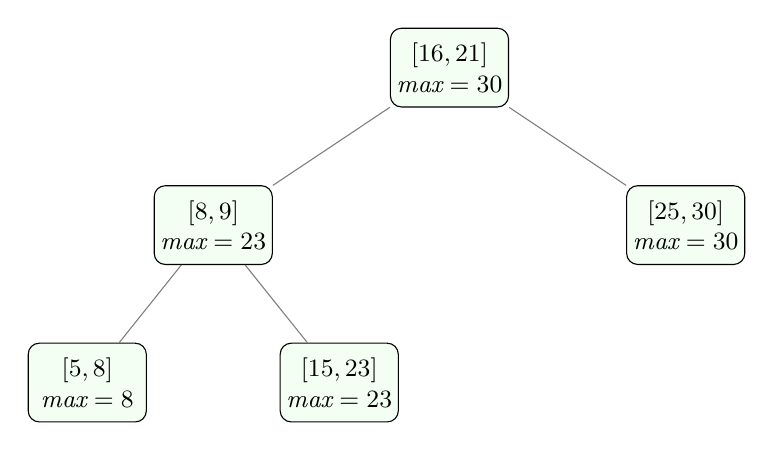
\begin{tikzpicture}[
  every node/.style={font=\small},
  inode/.style={draw, rounded corners, minimum width=15mm, minimum height=10mm,
    fill=green!5, align=center, inner sep=2pt},
  edge/.style={draw, gray}]
  \node[inode] (r) at (0,0) {$[16,21]$\\ \textit{max}\,$=30$};
  \node[inode] (l) at (-3,-2) {$[8,9]$\\ \textit{max}\,$=23$};
  \node[inode] (rr) at (3,-2) {$[25,30]$\\ \textit{max}\,$=30$};
  \node[inode] (ll) at (-4.6,-4) {$[5,8]$\\ \textit{max}\,$=8$};
  \node[inode] (lr) at (-1.4,-4) {$[15,23]$\\ \textit{max}\,$=23$};
  \draw[edge] (r)--(l); \draw[edge] (r)--(rr);
  \draw[edge] (l)--(ll); \draw[edge] (l)--(lr);
\end{tikzpicture}
\end{center}

Check the root: the high endpoints in the whole tree are
$21, 9, 30, 8, 23$; the biggest is $30$, and indeed the root's
\texttt{max} is $30$. Check node $[8,9]$: its subtree holds $[8,9], [5,8],
[15,23]$, high endpoints $9, 8, 23$, max $= 23$. \checkmark

\subsection{\texttt{INTERVAL-SEARCH}: the one clever step}

Now \textbf{step 4}, the new operation. We want to find any interval overlapping
a query $i$. Start at the root and, at each node $x$, decide whether to go left or
right. Here is the rule, and it is the whole trick:

\begin{algorithm}[H]
\caption{\textsc{Interval-Search}$(T, i)$ --- find an interval overlapping $i$}
\KwIn{interval tree $T$ and a query interval $i$}
\KwOut{a node whose interval overlaps $i$, or \texttt{NIL} if none does}
$x \gets T.\mathit{root}$\;
\While{$x \ne T.\mathit{NIL}$ \textbf{and} $i$ does not overlap $x.\mathit{int}$}{
  \eIf{$x.\mathit{left} \ne T.\mathit{NIL}$ \textbf{and} $x.\mathit{left}.\mathit{max} \ge i.\mathit{low}$}{
    $x \gets x.\mathit{left}$\tcp*{a left interval might still reach $i$}
  }{
    $x \gets x.\mathit{right}$\;
  }
}
\Return $x$\;
\end{algorithm}

Read the branch carefully. At node $x$, if $x$'s own interval overlaps $i$ we are
done and the loop stops. Otherwise we go \emph{left} exactly when the left
subtree exists and its \texttt{max} (the farthest-right endpoint anywhere on the
left) is at least $i.\mathit{low}$ --- meaning some interval down the left
\emph{might} reach far enough right to touch $i$. If even the leftmost,
farthest-reaching interval cannot reach $i.\mathit{low}$, there is no point
looking left; go right instead.

\begin{intuitionbox}
The \texttt{max} field is acting like a periscope. Standing at $x$, you cannot
see the individual intervals buried in the left subtree, but \texttt{max} lets
you see the \emph{rightmost reach} of the entire left subtree in one glance. If
that rightmost reach falls short of where your query begins
($x.\mathit{left}.\mathit{max} < i.\mathit{low}$), the entire left subtree is
hopeless and you can discard it without looking. That is how one number prunes
half the tree.
\end{intuitionbox}

\begin{labbox}
Let us run \textsc{Interval-Search} for the query $i = [22, 25]$ on the tree
above. ($i$ starts at $22$, so $i.\mathit{low} = 22$, $i.\mathit{high} = 25$.)

\textbf{At root $[16,21]$.} Overlap? We need $16 \le 25$ (yes) \emph{and}
$22 \le 21$ (no). Not overlapping. Now the branch: the left child is $[8,9]$ with
$\mathit{max} = 23$. Is $23 \ge i.\mathit{low} = 22$? Yes --- so something on the
left \emph{might} reach $22$. Go left to $[8,9]$.

\textbf{At node $[8,9]$.} Overlap with $[22,25]$? Need $8 \le 25$ (yes) and
$22 \le 9$ (no). No overlap. Branch: left child is $[5,8]$ with $\mathit{max} =
8$. Is $8 \ge 22$? No. So abandon the left subtree --- nothing there reaches
$22$ --- and go right to $[15,23]$.

\textbf{At node $[15,23]$.} Overlap with $[22,25]$? Need $15 \le 25$ (yes) and
$22 \le 23$ (yes). \textbf{Overlap! Return $[15,23]$.}

And indeed $[15,23]$ and $[22,25]$ share the points $22$ and $23$. Notice the
periscope at work: at node $[8,9]$ we threw away the entire left subtree using a
single comparison $8 \ge 22$, never inspecting $[5,8]$ directly.

\begin{center}
\begin{tikzpicture}[
  every node/.style={font=\small},
  inode/.style={draw, rounded corners, minimum width=15mm, minimum height=10mm,
    fill=green!5, align=center, inner sep=2pt},
  visited/.style={draw=quotientorange, line width=1pt, fill=quotientorange!18},
  found/.style={draw=targetgreen, line width=1.2pt, fill=targetgreen!20},
  pruned/.style={draw=gray!50, fill=gray!8, text=gray},
  edge/.style={draw, gray}]
  \node[inode, visited] (r) at (0,0) {$[16,21]$\\ \textit{max}\,$=30$};
  \node[inode, visited] (l) at (-3,-2) {$[8,9]$\\ \textit{max}\,$=23$};
  \node[inode] (rr) at (3,-2) {$[25,30]$\\ \textit{max}\,$=30$};
  \node[inode, pruned] (ll) at (-4.6,-4) {$[5,8]$\\ \textit{max}\,$=8$};
  \node[inode, found] (lr) at (-1.4,-4) {$[15,23]$\\ \textit{max}\,$=23$};
  \draw[edge] (r)--(l); \draw[edge] (r)--(rr);
  \draw[edge, gray!50] (l)--(ll); \draw[edge] (l)--(lr);
\end{tikzpicture}
\end{center}

Orange marks the nodes the search visits for $i = [22,25]$; green is the
overlap it returns; the grayed-out $[5,8]$ is pruned by the periscope
($\mathit{max} = 8 < 22$) and never touched.
\end{labbox}

\begin{figure}[h]
\centering
\begin{tikzpicture}[font=\small]
  % Title centered above diagram
  \node[font=\footnotesize\scshape, text=gray!70!black] at (5.7, 4.4) {Geometric Intervals on the Real Line};
  
  % Number axis
  \draw[->, thick, gray!70] (-0.5, 0) -- (12.2, 0) node[right, font=\scriptsize] {$x$};
  \foreach \tick in {0, 5, 10, 15, 20, 25, 30} {
    \draw[gray!60] (\tick*0.38, 0.08) -- (\tick*0.38, -0.08) node[below, font=\tiny] {\tick};
  }

  % [5, 8] (Pruned)
  \draw[draw=gray!50, fill=gray!8, dashed, thick, rounded corners=1pt] (5*0.38, 0.5) rectangle (8*0.38, 0.85);
  \node[gray!60!black, font=\tiny] at (6.5*0.38, 0.675) {$[5,8]$};
  \node[gray!55!black, font=\tiny, above=1pt] at (6.5*0.38, 0.85) {pruned: $\mathit{max}=8 < 22$};

  % [8, 9]
  \draw[draw=quotientorange, fill=quotientorange!20, thick, rounded corners=1pt] (8*0.38, 1.35) rectangle (9*0.38, 1.7);
  \node[quotientorange!90!black, font=\tiny, above=1pt] at (8.5*0.38, 1.7) {$[8,9]$};

  % [15, 23] (Overlaps!)
  \draw[draw=targetgreen, fill=targetgreen!30, very thick, rounded corners=1pt] (15*0.38, 2.05) rectangle (23*0.38, 2.45);
  \node[targetgreen!90!black, font=\tiny\bfseries] at (19*0.38, 2.25) {$[15,23]$ (OVERLAP!)};

  % [16, 21] (Root)
  \draw[draw=quotientorange, fill=quotientorange!20, thick, rounded corners=1pt] (16*0.38, 2.8) rectangle (21*0.38, 3.15);
  \node[quotientorange!90!black, font=\tiny] at (18.5*0.38, 2.975) {Root $[16,21]$ (miss)};

  % [25, 30]
  \draw[draw=gray!60, fill=gray!15, thick, rounded corners=1pt] (25*0.38, 2.8) rectangle (30*0.38, 3.15);
  \node[gray!70!black, font=\tiny] at (27.5*0.38, 2.975) {$[25,30]$};

  % Query interval i = [22, 25]
  \draw[draw=sourceblue, fill=sourceblue!25, very thick, rounded corners=1pt] (22*0.38, 3.55) rectangle (25*0.38, 3.9);
  \node[sourceblue!90!black, font=\scriptsize\bfseries, above=1pt] at (23.5*0.38, 3.9) {Query $i=[22,25]$};

  % Overlap band
  \draw[dashed, targetgreen, thick] (22*0.38, 3.55) -- (22*0.38, 2.05);
  \draw[dashed, targetgreen, thick] (23*0.38, 3.55) -- (23*0.38, 2.05);
  \fill[targetgreen!20, opacity=0.5] (22*0.38, 2.05) rectangle (23*0.38, 2.45);
  \node[targetgreen!80!black, font=\tiny, right=2pt] at (23*0.38, 2.25) {overlap $[22,23]$};
\end{tikzpicture}
\caption{The geometry of an interval overlap query. For query $i = [22, 25]$, the search starts at root $[16, 21]$ (which misses $i$ as $21 < 22$). The left child has $\mathit{max}=23 \ge 22$, proving that the left branch can reach $i.\mathit{low}$. Following the left branch discovers the overlapping interval $[15, 23]$ in $O(\log n)$ time, safely bypassing $[5, 8]$ whose reach $\mathit{max}=8$ falls short.}
\label{ch14:fig-interval-query-geometry}
\end{figure}

\subsection{Why the periscope never lies}

It is not obvious that this greedy left/right choice can never miss an existing
overlap. What if we go left and the only overlapping interval was actually on the
right? The following lemma rules that out, and its proof is a small gem worth
sitting with.

\begin{lemma}[Interval search is correct, CLRS Theorem 14.2]
\label{ch14:interval-correct}
In \textsc{Interval-Search}, if the algorithm steps to a child, then that child's
subtree contains an interval overlapping $i$ \emph{whenever the whole tree
does}. Consequently, if some interval in $T$ overlaps $i$, the algorithm returns
one; otherwise it returns \texttt{NIL}.
\end{lemma}

\begin{proof}[Gentle proof]
Each iteration that does not stop sends us either left or right. We show that in
each case, we never abandon an overlap that exists.

\textbf{Case 1: we go right.} We only go right when the left child is missing, or
$x.\mathit{left}.\mathit{max} < i.\mathit{low}$. Take the interesting subcase,
$x.\mathit{left}.\mathit{max} < i.\mathit{low}$. By definition,
$x.\mathit{left}.\mathit{max}$ is the largest high endpoint anywhere in the left
subtree. So \emph{every} interval $i'$ in the left subtree has
$i'.\mathit{high} \le x.\mathit{left}.\mathit{max} < i.\mathit{low}$, i.e.\
$i'.\mathit{high} < i.\mathit{low}$ --- it ends strictly before $i$ begins. By
Definition~\ref{ch14:overlap-def}, no such $i'$ can overlap $i$. The left subtree
is genuinely empty of overlaps, so discarding it loses nothing. Going right is
safe.

\textbf{Case 2: we go left.} We go left when
$x.\mathit{left}.\mathit{max} \ge i.\mathit{low}$. So the left subtree contains
\emph{some} interval $i'$ with $i'.\mathit{high} \ge i.\mathit{low}$ (the one
achieving the max). That is half of the overlap condition. We must rule out the
danger that, despite a promising left subtree, the only true overlap was sitting
on the \emph{right}, and by going left we walk away from it.

Here is where the tree's sorting saves us. The tree is keyed on \emph{low}
endpoints. Consider that left-subtree interval $i'$ with
$i'.\mathit{high} \ge i.\mathit{low}$. If $i'$ overlaps $i$, we are home --- the
left subtree contains an overlap and going left is correct. If $i'$ does
\emph{not} overlap $i$, then since $i'.\mathit{high} \ge i.\mathit{low}$ already
holds, the other half of overlap must fail:
$i.\mathit{high} < i'.\mathit{low}$. But $i'$ is in the left subtree, and the
tree is sorted by low endpoint, so \emph{every} interval $i''$ to the right of
$i'$ (which includes the entire right subtree of $x$, and $x$ itself) has
$i''.\mathit{low} \ge i'.\mathit{low} > i.\mathit{high}$. Such an $i''$ starts
\emph{after} $i$ ends, so it cannot overlap $i$ either (Figure~\ref{ch14:fig-case2}).
Hence no overlap lives on
the right; if one exists at all it must be in the left subtree. Going left is
safe.

In both cases we move toward a subtree that still contains an overlap whenever
one exists. Since the loop also stops the moment $x$ itself overlaps, by the time
we reach \texttt{NIL} we have correctly concluded no overlap exists. \qedhere
\end{proof}

\begin{walkbox}
Take the decisive line of Case 2 on your walk: ``if $i'$ does not overlap but
$i'.\mathit{high} \ge i.\mathit{low}$, then $i.\mathit{high} < i'.\mathit{low}$,
and so everything to the right of $i'$ starts even later and also misses $i$.''
Draw two intervals on a number line where $i'.\mathit{high} \ge i.\mathit{low}$
yet they do not overlap. What must be true of their starts? Now slide a third
interval even farther right. See why it cannot rescue the overlap? That picture
\emph{is} the proof.
\end{walkbox}

\begin{figure}[H]
\centering
\begin{tikzpicture}[font=\small, >={Stealth[length=2mm]}]
  \draw[->] (-0.3,0) -- (9.3,0);
  % query i
  \draw[sourceblue, line width=2.2pt] (1.0,0.55) -- (3.5,0.55)
     node[midway, above, sourceblue] {$i$};
  \draw[gray, dashed] (3.5,0.65) -- (3.5,-1.4);
  \node[sourceblue, below] at (3.5,-1.4) {$i.high$};
  % i' reaches back past i.low but starts after i.high
  \draw[targetgreen, line width=2.2pt] (4.3,0.0) -- (5.2,0.0)
     node[midway, above, targetgreen] {$i'$};
  \draw[gray, dashed] (4.3,0.1) -- (4.3,-1.4);
  \node[targetgreen, below] at (4.3,-1.4) {$i'.low$};
  % a farther-right interval i''
  \draw[trapred, line width=2.2pt] (6.0,-0.45) -- (7.6,-0.45)
     node[midway, below=2pt, trapred] {$i''$ (farther right)};
\end{tikzpicture}
\caption{Case 2 of the correctness proof. If $i'$ does not overlap $i$ yet
$i'.high\ge i.low$, then $i.high < i'.low$: $i'$ begins to the right of where
$i$ ends. Any $i''$ sorted after $i'$ begins even farther right, so it cannot
overlap $i$ either. No overlap can hide on the right.}
\label{ch14:fig-case2}
\end{figure}

Since each iteration descends one level and the tree has height $O(\lg n)$,
\textsc{Interval-Search} runs in $O(\lg n)$ time. Insert and delete are
$O(\lg n)$ by the maintenance theorem. We have built a second, completely
different data structure with the same four-step recipe and the same locality
trick.

\begin{complexitybox}
Interval tree (red-black base, $n$ intervals):
\begin{center}
\begin{tabular}{ll}
\toprule
Operation & Worst-case time \\
\midrule
\texttt{INTERVAL-INSERT}, \texttt{INTERVAL-DELETE} & $O(\lg n)$ \\
\texttt{INTERVAL-SEARCH}$(i)$ (find one overlap) & $O(\lg n)$ \\
report \emph{all} $k$ overlaps & $O((k+1) \lg n)$ \\
extra space & $O(n)$ (one \texttt{max} per node) \\
\bottomrule
\end{tabular}
\end{center}
``Find all $k$ overlaps'' is just: find one, delete it from a copy, repeat ---
each round is $O(\lg n)$, there are $k$ successful rounds plus one final round
that reports ``no more,'' giving $O((k+1)\lg n)$; or, better, recurse using the
\texttt{max} fields to prune (Exercise~\ref{ch14:ex-alloverlaps}).
\end{complexitybox}

\begin{aestheticbox}
Interval trees are everywhere there is a notion of ``range'' and a need to detect
clashes fast. Calendar apps check whether a proposed meeting collides with any
existing one. Network routers and firewalls match a packet's address against
ranges of allowed addresses. Genome browsers find which genes overlap a region of
a chromosome --- a query that runs millions of times over datasets with hundreds
of millions of features, where the difference between $O(\lg n)$ and $O(n)$ per
query is the difference between interactive and useless.
\end{aestheticbox}

\section{A Field Guide to Augmentation}

Notice what made both examples work. In each case we found a field
that summarizes a subtree and is computable from a node plus its children's
fields. Once you have that, the theorem hands you maintenance for free, and your
job shrinks to designing the clever query (\texttt{SELECT}/\texttt{RANK}, or the
left/right periscope). Here is a small catalog of fields that pass the locality
test, to train your eye:

\begin{center}
\begin{tabular}{lll}
\toprule
Field at node $x$ & Local formula & Buys you \\
\midrule
\texttt{size} & $\ell.\mathit{size} + r.\mathit{size} + 1$ & rank, select, percentile \\
\texttt{sum} & $\ell.\mathit{sum} + r.\mathit{sum} + x.\mathit{key}$ & subtree / prefix sums \\
\texttt{min} & $\min(x.\mathit{key}, \ell.\mathit{min}, r.\mathit{min})$ & range minimum \\
\texttt{max-high} & $\max(x.\mathit{high}, \ell.\mathit{max}, r.\mathit{max})$ & interval overlap \\
\texttt{height} & $1 + \max(\ell.\mathit{height}, r.\mathit{height})$ & subtree height \\
\bottomrule
\end{tabular}
\end{center}

Each one reads only off the node and its two children, so each one is free to
maintain. The art is matching the field to the question.

\begin{trapbox}
A subtle failure: not every useful field is local, and you must check rather than
hope. ``Number of nodes within distance $d$ of $x$ in key-value'' or ``the median
of my subtree'' do \emph{not} obey the locality condition --- a child's median tells
you almost nothing about the parent's median. When a field fails the test, you
have two moves: enrich it into something that \emph{is} local (store a sorted
summary, a count, a histogram), or accept that this particular field will cost
more than $O(\lg n)$ to keep current. Never assume; write down the formula and
see whether only the children appear.
\end{trapbox}

\begin{recoverybox}
If your head is full, here is the one sentence to keep. \textbf{To augment a
balanced tree, add a field that each node can compute from itself and its two
children; the rebalancing machinery will then maintain it for free, and you spend
your cleverness only on the query.} Order-statistic trees and interval trees are
two instances of that one sentence.
\end{recoverybox}

\section*{A Closing Picture}

Look back at what we actually did in this chapter. We did not invent
two new data structures. We took \emph{one} structure we already trusted --- the
red-black tree --- and, twice, taught it to answer a new family of questions by
storing a single extra number per node and writing one clever query. The
maintenance theorem is the reason this is a repeatable craft rather than a stroke
of luck each time: as long as your extra information is \emph{local} --- readable
from a node and its children --- the expensive part (keeping it correct under
insertion, deletion, and rebalancing) is handled for you, automatically, at no
asymptotic cost.

Carry that stance into the rest of the book and into real
systems. When a problem looks like it needs a bespoke structure, pause and ask:
\emph{is there a balanced tree underneath, and a small local summary I could bolt
on to answer this?} Surprisingly often, the answer is yes.

Up to this point in the book, our main lever for speed has been data structure design:
organizing elements so that queries can drill straight down to the answer in
$O(\lg n)$ time. In Part~IV, we turn from organizing stored data to the structure of
algorithmic decisions themselves. In \textbf{Chapter~15 (Dynamic Programming)}, we
encounter problems where subproblems overlap and repeat, learning how to record
subproblem solutions in a table to collapse exponential search spaces into fast
polynomial-time algorithms.

\section{Exercises}

\begin{exercise}[Warm-up: trace by hand]
Build an order-statistic tree (you may draw any balanced shape) on the keys
$\{3, 8, 12, 19, 22, 27, 35\}$, labelling each node with its \texttt{size}.
Then run \textsc{OS-Select}$(\mathit{root}, 5)$ step by step, and separately
compute \textsc{OS-Rank} of the node holding key $22$. Confirm the two answers
are consistent (i.e.\ \texttt{SELECT} and \texttt{RANK} invert each other on this
key).
\end{exercise}

\begin{exercise}[The forgotten subtraction]
A classmate writes \textsc{OS-Select} but recurses right with the unchanged index
$i$ instead of $i - r$. On the seven-node tree from
Section~\ref{ch14:sec-ostree}, trace their buggy code for the query $i = 6$ and
show that, because the inflated index is never shrunk on a right turn, the
recursion walks off the right end of the tree (it reaches a \texttt{NIL} child
asking for an index larger than any subtree can hold). What is the correct
answer? Explain in one sentence why dropping the subtraction breaks the meaning
of $i$.
\end{exercise}

\begin{exercise}[Maintaining size through a rotation]
Suppose a left rotation is performed at a node $x$ whose subtrees have sizes
$\alpha = 6$ (left of $x$), $\beta = 3$, $\gamma = 5$ (with $\beta, \gamma$ the
subtrees of $x$'s right child $y$, as in the figure). Compute every
\texttt{size} field before and after the rotation, and verify the total node
count is unchanged.
\end{exercise}

\begin{exercise}[Counting smaller elements]
Using an order-statistic tree, give an $O(\lg n)$ algorithm \texttt{COUNT-LESS}$(k)$
that returns how many keys in the tree are strictly less than a given value $k$
(where $k$ need not be present in the tree). Sketch the algorithm and argue its
running time.
\end{exercise}

\begin{exercise}[Does the field stay local?]
For each proposed node field, write down its formula in terms of the node and its
children, and state whether it satisfies the locality hypothesis of
Theorem~\ref{ch14:augment-theorem}. (a) the number of \emph{red} nodes in the
subtree; (b) the depth of the node (its distance from the root); (c) the sum of
all keys in the subtree; (d) the second-smallest key in the subtree.
\end{exercise}

\begin{exercise}[Overlap by hand]
On the five-interval tree of Section~\ref{ch14:sec-interval}, run \textsc{Interval-Search}
for the query $i = [11, 14]$. Show which node you visit at each step, which
branch you take and why (cite the \texttt{max} comparison), and the final
result.
\end{exercise}

\begin{exercise}[The point-stabbing query]
Specialize interval search to a single point: given a number $p$, find any
interval in the tree that contains $p$. Show that this is just
\textsc{Interval-Search} with the degenerate query interval $[p, p]$, and rewrite
the overlap test for this case. What does the \texttt{max} pruning rule become?
\end{exercise}

\begin{exercise}[Report all overlaps]
\label{ch14:ex-alloverlaps}
Modify interval search to return \emph{all} $k$ intervals overlapping a query $i$,
rather than a single match. Argue that a careful recursion (descending left only when
$x.\mathit{left}.\mathit{max} \ge i.\mathit{low}$, and right only when
$x.\mathit{int}.\mathit{low} \le i.\mathit{high}$) finds all of them, and that its
running time is $O((k+1)\lg n)$.
\end{exercise}

\begin{exercise}[A new augmentation: subtree sum]
Augment a balanced BST so that each node stores the \texttt{sum} of all keys in
its subtree. (a) Give the local formula and confirm it passes
Theorem~\ref{ch14:augment-theorem}. (b) Give an $O(\lg n)$ operation
\texttt{SUM-LESS}$(k)$ returning the sum of all keys strictly less than $k$.
(c) Explain how \texttt{sum} is fixed up during a left rotation.
\end{exercise}

\begin{exercise}[Challenge: dynamic minimum-gap]
You maintain a dynamic set of distinct numbers in a balanced tree and want to
support \texttt{MIN-GAP}, returning the smallest difference between any two
adjacent numbers (in sorted order) currently in the set. Design an augmentation
that supports \texttt{INSERT}, \texttt{DELETE}, and \texttt{MIN-GAP} in
$O(\lg n)$. \emph{Hint: at each node store three local summaries --- the minimum
key, the maximum key, and the minimum adjacent gap within the subtree --- and write
the formula combining a node with its two children. Check it is local.}
\end{exercise}

\begin{exercise}[Challenge: why not store rank directly?]
Argue carefully that storing each node's global rank (its position in sorted
order) as a field cannot be maintained in $o(n)$ time per insertion in the worst
case. Then explain in one paragraph how the \texttt{size} field sidesteps this
exact difficulty while still answering rank queries in $O(\lg n)$.
\end{exercise}
